
\section{Mathematical Background}

Here, we will introduce some basic linear algebra, optimization, and machine learning concepts that will be useful particularly in Chapters~\ref{chapter:autoreject} and \ref{chapter:alphacsc} on \emph{autoreject} and \emph{alphacsc}.

\subsection{Norms}
Informally speaking, a norm is used to measure the length or size of a vector. It must also satisfy some properties, but it will not be of concern for us in this thesis. It is sufficient to know the mathematical expression, how it behaves, and the physical property that it captures.
\theoremstyle{definition}
\newtheorem{definition}{Definition}[chapter]
%
%
\vspace{\parskip}
\begin{definition}{($\ell_p$ norm.)}
For $1 \leq p < \infty$, the $\ell_p$ norm of a vector $x$ is defined by:
\begin{equation}
\|x\|_p = \Big(\sum_n \ \lvert x_n \rvert^p \Big)^{1/p}.
\end{equation}
\label{def:lp_norm}
\end{definition}
%
%
\begin{definition}{($\ell_0$ ``norm''.)}
The $\ell_0$ ``norm'' of a vector $x$ is defined by:
\begin{equation}
\|x\|_0 = \sum_n \ \lvert x_n \rvert^0.
\end{equation}
\label{def:l0_norm}
\end{definition}
%
%
\vspace{\parskip}
\begin{definition}{($\ell_\infty$ norm.)}
The $\ell_\infty$ norm of a vector $x$ is defined by:
\begin{equation}
\|x\|_{\infty} = \sup_n \ \lvert x_n \rvert.
\end{equation}
\end{definition}
As we are taking the supremum, this norm is sensitive to large values in the vector, which is needed for measuring artifacts.
%
%
\vspace{\parskip}
\begin{definition}{(Frobenius norm.)}
The Frobenius norm of a real-valued matrix $A$ is defined by:
\begin{equation}
\|A\|_{\mathrm{Fro}} = \| \mathrm{vec}(A) \|_2 = \sqrt{\mathrm{trace}(AA^\top)}.
\end{equation}
%
The Frobenius norm is a matrix norm that is simply the $\ell_2$ vector norm of the vectorized matrix $\mathrm{vec}(A)$.

\end{definition}

\subsection{Cross validation}

Cross validation is a statistical technique to estimate how well a predictive model will \emph{generalize} to unseen data. We will be using cross validation in our \emph{autoreject} work presented in Chapter~\ref{chapter:autoreject}. Cross validation is normally performed by partitioning the data into two and learning the model from one part (typically the larger one) while validating it on the other. These two parts are known as the \emph{training} and the \emph{validation} sets respectively. In order to get reliable estimates of the model performance, this procedure is repeated multiple times and the results are averaged.

Depending on the data, different types of partitioning schemes are preferred. In \emph{K-fold} cross validation, the data is divided into $K$ equal parts (with or without shuffling the samples), where $K - 1$ parts are used for training and the $K$th part is used for validation. In a \emph{stratified} cross-validation scheme, the partitions are done such that each partition has roughly equal number of samples from each class.

\paragraph{Underfitting and overfitting: } When a statistical model explains the data too closely, it results in overfitting. An overfitted model is often unable to make accurate predictions of unseen data. The converse is also true. When the model is unable to explain much structure in the data, it is known as underfitting. As we will see in Chapter~\ref{chapter:autoreject}, these concepts are closely related to model selection. The goal is typically to find a model with hyperparameters (\textit{e.g.} regularization constant or the width of a Gaussian) that neither underfit nor overfit. We will next discuss some strategies to tune these hyperparameters.

\paragraph{Grid search: } Quite often, a machine learning model contains hyperparameters which need to be tuned to get optimal performance on the data. This tuning to select the best model can be done automatically using cross validation. The idea is to exhaustively search over the parameter space by trying an equally spaced grid of hyperparameters that the model can admit and selecting the one which performs the best.

\paragraph{Random search: } Sometimes grid search is too slow, and it is better to try parameters sampled randomly without a considerable loss in performance. This is known as random search.

\paragraph{Nested cross validation: } When cross validation has been used for finding the best model, a separate unseen partition, known as the \emph{test} set, is needed to assess the generalization power of the best model. The test set must be different from all the data that was seen so far, including \emph{both} the training and the validation sets. This is done to avoid a circularity bias as noted in \citet{varoquaux2017assessing, cawley2010over,friedman2001elements}.
Therefore a nested cross-validation scheme is necessary where in each outer loop, the best model is found, and its performance is computed.

\subsection{Bayesian optimization}


\begin{figure}[htb]
\begin{center}
   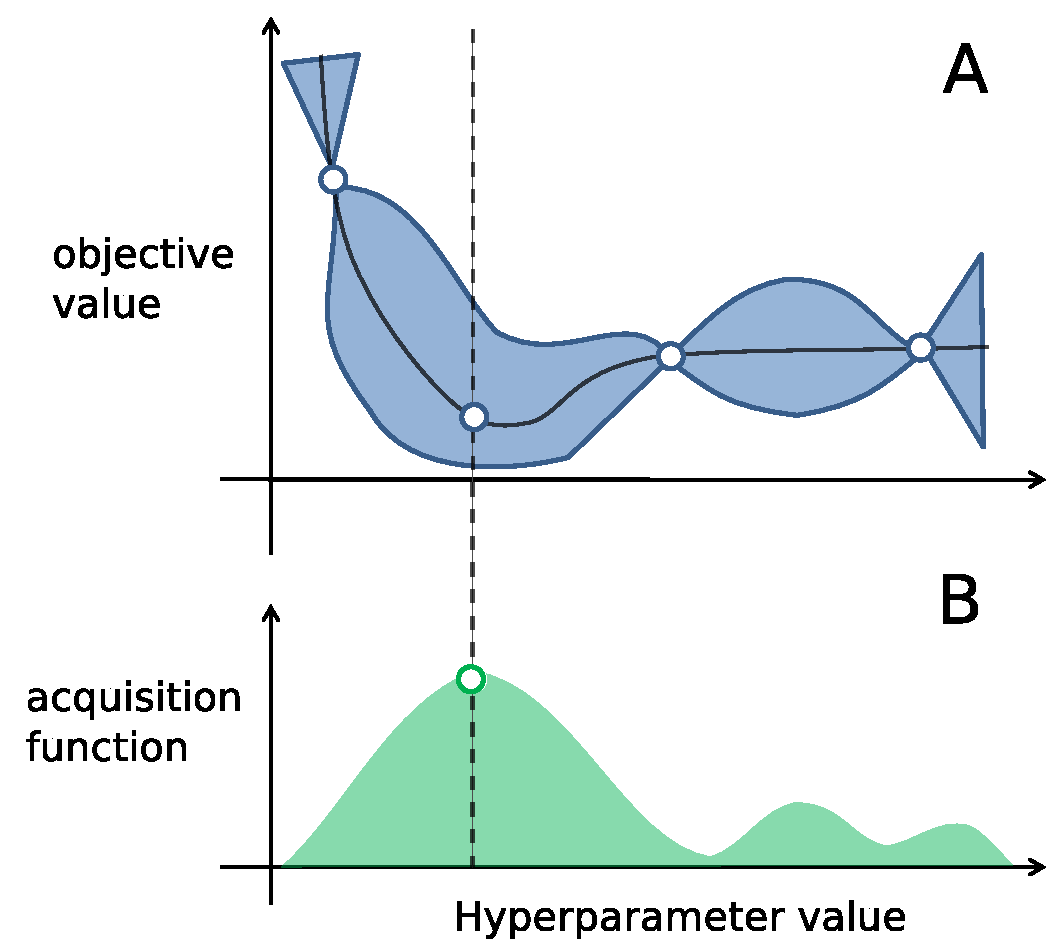
\includegraphics[width=0.7\linewidth]{figures/bayes_opt.pdf}
\end{center}
   \caption[Bayesian optimization for parameter tuning]{An illustration of how Bayesian optimization is used to sequentially select new points (A) Gaussian process to estimate uncertainties on the objective function for the parameter space, and (B) Acquisition function to balance the ``exploration'' \emph{vs} ``exploitation'' dilemma.}
   \label{fig:bayes_opt}
\end{figure}

Sometimes grid search is too slow and random search is not sufficiently accurate for tuning hyperparameters. In such cases, one may have to rely on more efficient black box optimization techniques. Bayesian optimization~\citep{snoek2012practical} is one such method which is a sequential method, and iteratively improves the objective function that we are optimizing.

Since these methods must work for any kind of function which may not be necessarily convex, we cannot rely on classical gradient based methods. The central idea in these types of methods is to search as much of the hyperparameter space as possible, while keeping a record of the objective values evaluated so far. A very natural strategy is therefore to either search around points which have high objective values, or in those areas where it is unknown. This is indeed a case for the classic  ``exploration'' \emph{vs.} ``exploitation'' dilemma that is well known in computer science.

In order solve this dilemma, an \emph{acquisition function} is typically used, as shown in Figure~\ref{fig:bayes_opt}. While the ``exploitation'' component of this function is easy to compute from the objective values, in order to compute the ``exploration'' component, we can fall back upon \acp{GP}~\citep{rasmussen2004gaussian}. Given the points evaluated until now, a \ac{GP} can be used to estimate the uncertainty in the rest of the search space. 

\subsection{Dictionary learning}
\label{sec:background_dict_learning}

As we described in Section~\ref{sec:representation_learning}, we will be using the framework of dictionary learning to automatically mine prototypical waveforms from neural time series. Our work will build upon existing work in shift-invariant sparse coding and data decomposition methods. In this section, I introduce some concepts, which are well known in the dictionary learning community, but might be useful for anyone not so familiar with the area.

\paragraph{Dictionaries and sparsity:} A \emph{dictionary} is a set of \emph{atoms} (also known as filters sometimes) which can be combined with certain \emph{coefficients} (or activations) to approximate the data. 
The atoms could be fixed (for example wavelets or Gabor), or they could be learned directly from the data itself. As such, there is no requirement of orthogonality on the atoms. 
To learn a representation of the data boils down to estimating the coefficients used in the approximation, which are often assumed to be sparse, \emph{i.e.}, they have very few non-zero values. 
The learning algorithm is therefore called \emph{sparse coding} and the coefficients learned are known as the \emph{sparse code}.

Sparsity can be promoted by using an $\ell_0$ or $\ell_1$ penalty, which helps maintain a compact representation. Note that the $\ell_0$ ``norm'' simply counts the number of elements in the vector (c.f., Definition~\ref{def:l0_norm}) , therefore adding it as a regularizer will favour solutions that have fewer non-zero elements. In the traditional approach, it is quite common to start off with an \emph{overcomplete} dictionary, \emph{i.e.,} to have more atoms than would be needed, and only estimate the coefficients (keeping the atoms fixed). This can be done, for example, using matching pursuit~\citep{mallat1993matching}, which is a greedy algorithm for sparse approximations.

\paragraph{Learning atoms:} It is easy to see that the overcomplete approach is memory intensive as it has more atoms that necessary, but also this approach requires making assumptions about the shape of the atoms in the dictionary. Nowadays, it is more common to learn the atoms in addition to the sparse code, which is known as \emph{dictionary learning}. Dictionary learning can be thought of as a data decomposition method (or matrix factorization) technique (like \ac{PCA} or \ac{ICA}), but with a sparse regularization. As for obtaining sparse solutions, the goal is to have as few non-zero coefficients as possible, an $\ell_0$ penalty is typically used. However, this leads to a non-convex formulation of the problem. One strategy to deal with this is using a convex relaxation by replacing the non-convex $\ell_0$ penalty using the $\ell_1$ penalty which is convex. 
This is often a reasonable approximation which makes the problem biconvex, and can therefore be solved by alternate minimization. Dictionary learning is now being used for denoising~\citep{elad2006image}, inpainting~\citep{mairal2009online}, and classification~\citep{mairal2009supervised}. 

\paragraph{Coding for shift invariance:}
In traditional dictionary learning, the signal or the image is divided into patches and these patches are used as samples for the learning. The main disadvantage of this method is that it results in redundant atoms that are shifted versions of each other. This is the reason a shift-invariant version of dictionary learning is needed. One of the earliest paper in this regard can be credited to \cite{lewicki1999coding}. In their work, the dictionary was fixed and the shift-invariance was encoded using convolutions. 
This is possible because the convolution operator is defined by an integration (correspondingly summation in the discrete domain) as below.
\vspace{\parskip}
%
\begin{definition}{(Convolution)}
\label{def:convolution}
A convolution of two functions $f$ and $g$ is written $f * g$ and computed as:
\begin{equation}
(f * g)(t) \triangleq \int_{-\infty}^{\infty} f(\tau)g(t-\tau) d\tau
\end{equation}
\end{definition}

In the discrete case where $f$ and $g$ are vectors with finite support $[0,..,M]$ and $[0,..,N]$ and $N > M$, this can be rewritten as
%
\begin{equation}
(f * g)[n] = \sum_{m=0}^{M-1} f[m]g[n-m],
\end{equation}
%
so that $f * g$ has a support of $[0,..,(N - M + 1)]$ if the edges are truncated. As we can see, if either $f$ or $g$ is zero padded, the other function can be shifted along these zeros yielding the same result.

As a result of the convolutional approach, the atoms learned are not redundant and the location of the atom is encoded in the activations. This type of approach is refered to as \ac{CSC} or shift-invariant dictionary learning in the literature. In practice, an overcomplete dictionary in the shape of a Toeplitz matrix is constructed by shifting the atoms across time. This is the same formulation which is still being used to code shift invariance even if the learning algorithms are more sophisticated now. More recent work by \cite{grosse2012shift} have made use of the Fourier transform to solve the problem in Frequency domain and compute an inverse transform of the learned dictionary in the end. Another approach that has proved to be quite efficient is the so-called predictive sparse coding which uses neural networks~\citep{kavukcuoglu2010learning}. It is hard to summarize all the work in this area, but it suffices to say that shift-invariant dictionary learning has been gaining popularity in audio signals, images, music, and now for neural data (See Section~\ref{sec:alphacsc_intro} for a more comprehensive list of references).

\subsection{Iterative solvers for convex problems}

Much of the dictionary learning techniques in literature leverage convex optimization methods, which are iterative techniques to solve minimization problems involving convex functions. In our \emph{alphacsc} work presented in Chapter~\ref{chapter:alphacsc}, we will also be using such methods. \ac{CSC} being a biconvex problem (\textit{i.e.,}  convex if either the atoms or the activations are fixed), is amenable to such methods.

Therefore, let us first recall what is a convex function before diving into the details of these methods.
\vspace{\parskip}
\begin{definition}{(Convex function)}
\label{def:convexity}
A function $f$ is convex if it satisfies
\begin{equation}
\forall x_1, x_2 \in X, \forall t \in [0, 1]: f(tx_1 + (1 - t)x_2) \leq tf(x_1) + (1 - t)f(x_2).
\end{equation}
\end{definition}

\begin{figure}[htb]
\begin{center}
   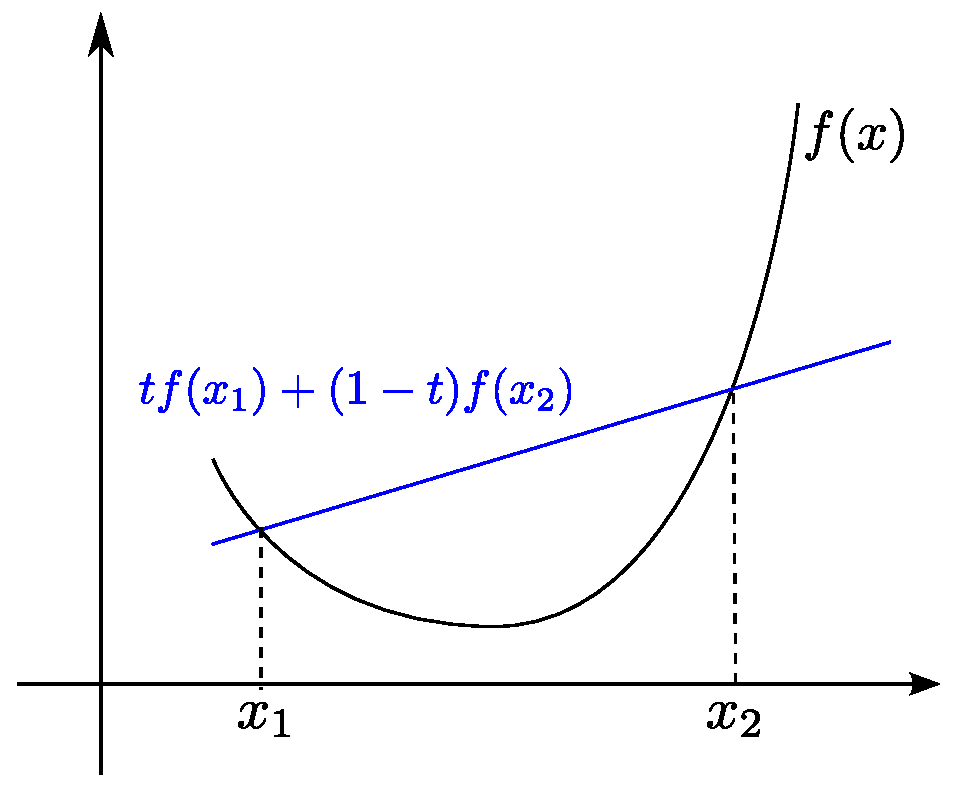
\includegraphics[width=0.5\linewidth]{figures/convex_functions.pdf}
\end{center}
   \caption[Graphical illustration of convexity]{A graphical illustration of Definition~\ref{def:convexity} for convex functions.}
   \label{fig:convexity}
\end{figure}

In other words, for any two points on the function, the line joining those two points lies above the graph of the function (as illustrated in Figure~\ref{fig:convexity}). A convex function lends itself to the property that the global minimum is also necessarily the local minimum. This concept can also be extended to define strong convexity which guarantees that the local minimum is not only the global minimum, but also it is unique.

Throughout the thesis, we will be solving unconstrained minimization problems of the form
\begin{equation}
x^{\star} = \argmin_x \|Ax - b\|_{2}^2 + \Omega(x),
\label{eq:linreg_minimize}
\end{equation}

%
where typically $A \in \mathbb{R}^{n \times p}$ is the design matrix with $n$ rows (samples) and $p$ columns (features), $x \in \mathbb{R}^p$, and $b \in \mathbb{R}^n$. A penalty or regularization term $\Omega(x)$ is added to prevent solutions that overfit. 
If there was no regularization term $\Omega(x)$, we could solve this in closed form and get $x^{\star} = {(A^{\top}A)}^{-1}A^{\top}b$. However, this can be computationally prohibitive as inverting $A^{\top}A$ is $\mathcal{O}(p^3)$, and iterative methods based on gradient descent are more efficient as they require only a matrix-vector dot product. These are what we shall refer to as \emph{solvers}. More importantly, these gradient based methods can work for arbitrary functions as long as we have access to the gradient (or even its approximation).

In gradient based methods, we make updates of the  form:
%
\begin{equation}
x_{k + 1} = x_{k} + \rho_k d_k,
\label{eq:update_term}
\end{equation}
%
where $\rho_k$ is a scalar which defines the step size and $d_k \in \mathbb{R}^p$ is the search direction.

\paragraph{Gradient descent: } In the case of gradient descent, the search direction $d_k$ is the negative gradient $-g(x_k)$ and the typical step size $\rho_k=1/L$ where $L$ is the Lipschitz constant of the gradient, which upper bounds the rate at which it changes. The intuition behind this method is that if we follow the negative gradient direction, we will progressively reach a point where the gradient is 0 and this corresponds to the minimum for convex functions.

However, often the regularization term $\Omega(x)$ is not smooth, and therefore it does not have a unique derivative at all points. In these cases, we must resort to proximal gradient methods.

\paragraph{Proximal algorithms: } An example of a non-smooth regularizer which is encountered in practice, and will also be used in our work, is the $\ell_1$ norm~\citep{tibshirani1996regression}. It induces sparsity using $\Omega(x) = \lambda \|x\|_1$, where $\lambda$ controls the sparsity level. The higher the $\lambda$, sparser the solution. In such situations, we can use what are known as proximal methods. The idea behind proximal methods is to take a gradient step using only the smooth part of the function, and then apply a proximal operator (which depends on the non-smooth part) on the resulting iterate. 

\vspace{\parskip}
\begin{definition}{(Proximal operator)}
A proximal operator associated with a convex function $f$ is defined as
\begin{equation}
\mathrm{prox}_f(v) = \argmin_x \bigg( f(x) + \frac{1}{2}\|x - v\|_2^2 \bigg).
\end{equation}
\end{definition}

The proximal operator can be thought of as a generalized projection operator~\citep{parikh2014proximal}. For the $\ell_1$ norm with $f(x)=\|x\|_1$, it is the soft thresholding function $\mathcal{S}_\lambda(\cdot)$ which induces sparsity, and is given by

\begin{equation}
\mathcal{S}_{\lambda}(v) = \begin{cases}
v - \lambda \quad \text{if }  v > \lambda, \\
0 \quad \hspace{22pt} \text{if } -\lambda \leq v < \lambda,\\
v + \lambda \quad \text{if } v < -\lambda.
\end{cases}
\end{equation}

The resulting algorithm is known as \ac{ISTA}~\citep{daubechies2004iterative, bach2012optimization}, which has a convergence rate of $\mathcal{O}(1/k)$ for $k$ iterations. Proximal algorithms are also helpful when dealing with constraints. For example, in Equation~\ref{eq:linreg_minimize}, if we had a norm-1 constraint $\|x\|_2^2 \leq 1$, this could be recast using an indicator function $i(\cdot)$:

\begin{equation}
i(x) = \begin{cases}
\infty \qquad \text{if } \|x\|_2^2 \leq 1 \\
0 \qquad \hspace{7pt}\text{if } \|x\|_2^2 > 1
\end{cases}
\end{equation}

In this case, the proximal operator can be shown to be the projection $\pi(x)$ on to the unit ball which is expressed as

\begin{equation}
\pi(x) = \frac{x}{\mathrm{max}(1, \|x\|_2)}.
\end{equation} 

This is what is known as \textit{projected gradient descent}. We will encounter such constraints in our dictionary learning problem in Section~\ref{sec:m-step}. It will be used to handle the scale ambiguity between the atoms and activations when performing optimization.

\paragraph{Acceleration:} Gradient descent has slow convergence due to oscillations if the condition number of $A$ is high as it leads to pathological curvature. A faster rate of convergence can be achieved using Nesterov accelerations~\citep{nesterov1983method}, which adds a momentum term to the update in Equation~\ref{eq:update_term}.
The momentum term takes into account the update vector from the past iterations so as to dampen the oscillatory behaviour observed in classical gradient descent and \ac{ISTA}. 
This results in an algorithm known as \ac{FISTA}~\citep{beck2009fast} which has a faster convergence rate of $\mathcal{O}(1/k^2)$. It has been proved theoretically that this is the fastest rate possible if we had access to only the gradient and function evaluations. The full algorithm is summarized in Algorithm~\ref{alg:fista}.

    \begin{algorithm}[htb]
      \begin{algorithmic}[1] %(regularization parameter), (number of EM iterations), (number of MCMC iterations)
      \REQUIRE Regularization: $\lambda \in \real_+$, Design matrix A, b
      \STATE $x_1=0=z_1, \beta_1=1$
        \FOR{$k=1$ to $K$}
          
          \STATE $x_{k+1} = \mathcal{S}_{\lambda/L}(z_k - \frac{1}{L}g(z_k))$ \textit{\color{blue} /* Proximal step */}
          \STATE $\beta_{k+1} = (1 + \sqrt{1 + 4(\beta_k)^2})/2$
          \STATE $z_{k + 1} = x_{k + 1} + \frac{\beta_k - 1}{\beta_{k + 1}}(x_{k + 1} - x_k)$ \textit{\color{blue} /* Momentum update */}
        \ENDFOR
        \RETURN $x_{K + 1}$
        \end{algorithmic}
        \caption{Fast iterative soft thresholding algorithm}
        \label{alg:fista}
    \end{algorithm}

% \paragraph{ADMM:} Convergence rate of $\mathcal{O}(1/k)$

\paragraph{Quasi-Newton methods:}
If in the updates of Equation~\ref{eq:update_term}, instead of using the negative gradient for the search direction, we used $d_k = -H^{-1}(x_k)g(x_k)$, with $H(x_k)$ being the Hessian, it would be known as Newton's method. As opposed to first order methods which use only gradient information, Newton-based methods also make use of the curvature. Newton's method has a locally quadratic convergence, but it may diverge when the current iterate is far from the optimum. Even if this is not the case, a Hessian that is not positive definite can also cause diverging behaviour. Therefore, the step size $\rho_k$ must be chosen carefully, for example using a line search strategy.

Of course, the Hessian is costly to compute and to invert, therefore quasi-Newton methods can be used which approximate it using a matrix $B_k$. Starting with $B_k = I$, we can update this matrix at each step using a cheap rank 1 or rank 2 correction. For instance, in the Broyden formula, we would do
\begin{equation}
B_{k+1} = B_k + vv^\top.
\end{equation}
The vector-vector outer product $vv^\top$ is the rank-1 correction in the above formula. The more advanced David-Fletcher-Powell formula uses a rank-2 correction and so does the \ac{BFGS} algorithm. When the entire Hessian matrix cannot be stored in memory, a limited memory version of BFGS~\citep{wright1999numerical} can be used where only a few vectors $v$ from the last few iterations are stored for the approximation.

\paragraph{Coordinate descent:}
In coordinate descent, we minimize one coordinate at a time. The idea behind coordinate descent is rather simple, yet it performs surprisingly well in practice. Thus  Equation~\ref{eq:update_term} would be coordinatewise, \textit{i.e.,} for each iteration, we would choose a coordinate $i_k$ and perform an update:

\begin{equation}
\begin{cases}
x^{(i)}_{k+1} = x^{(i)}_{k} - \rho^{(i)}_k g^{(i)}(x_k) \quad \text{if } i=i_{k+1}\\
x^{(i)}_{k+1} = x^{(i)}_{k} \hspace{80pt} \text{if } i \neq i_{k+1}
\end{cases}
\end{equation}

Of course, we could have also solved each coordinate in closed form instead of using gradients per coordinate. However, in this formulation, if the non-smooth part of the objective (typically the regularizer) is \emph{separable} (\textit{i.e.,} $f(x) = \sum_i f^{(i)}(x_i)$), it allows us to even extend it to proximal coordinate descent. While in coordinate descent, we iterate over the $p$ coordinates, each coordinate update is computationally less demanding than a full gradient update. The coordinates can be chosen either cyclically or at random. In \emph{block} coordinate descent, groups of coordinates are selected for updating rather than one coordinate at a time. It is what we will use for updating the atoms and activations in \emph{alphacsc} (Chapter~\ref{chapter:alphacsc}).

% \subsection{Interpolation schemes}
